%%%%%%%%%%%%%%%%%%%%%%%%%%%%%%%%%%%%%%%%%%%%%%%%%%%%%%%%
% Este é um documento que servirá de modelo para
% os relatórios feitos na disciplina Circuitos Digitais
% 2016-2
%%%%%%%%%%%%%%%%%%%%%%%%%%%%%%%%%%%%%%%%%%%%%%%%%%%%%%%%%

\PassOptionsToPackage{brazil,american}{babel}
\documentclass[12pt]{article}

\usepackage{sbc-template}
\usepackage[brazil,american]{babel}
\usepackage[utf8]{inputenc}

\usepackage{graphicx}
\usepackage{url}
\usepackage{float}
\usepackage{listings}
\usepackage{color}
\usepackage{todonotes}
\usepackage{algorithmic}
\usepackage{algorithm}
\usepackage{hyperref}
\usepackage{enumitem}
     
\sloppy

\title{Experimento 4\\
	Circuitos Combinacionais : Comparador de Palavras }

\author{Isaac Lopes, 12/0120801\\
	Lucas Mafra Chagas, 12/0126443 \\
	Marcelo Giordano Martins Costa de Oliveira,  12/0037301
}


\address{Dep. Ciência da Computação -- Universidade de Brasília (UnB)\\
	CiC 116351 - Circuistos Digitais - Turma C
	\email{\{giordano.marcelo, chagas.lucas.mafra, isaaclopinho\}@gmail.com}
}

\begin{document} 

\maketitle

 \begin{abstract}
   Write here a short summary of the report in English. This corresponds to the Experiment 7 report on combinational circuits, specifically the multiplexers.
 \end{abstract}
     
 \begin{resumo} 
  Escreva aqui um pequeno resumo do relatório. Este corresponde ao relatório do Experimento 7 sobre circuitos combinacionais, especificamente os multiplexadores.
 \end{resumo}


\section{Objetivos}
\label{sec:Objetivos}

Os objetivos do presente relatório são de usar o sistema Quartus II para a implementação de circuitos com comparadores de palavras binárias com as técnicas utilizadas em relatórios passados de simplificação e montagem.

\section{Materiais} 
\label{sec:Materiais}

\begin{itemize}
    \item software Quartus-II v13.0
\end{itemize}
\section{Introdução}
\label{sec:Introducao}

Um comparador é um circuito combinatório operativo. Ele permite comparar grandezas de dois números binarios.Um comprimento de uma palavra binária é o número de bits que a compõem.
\begin{figure}[H]
	\centering
	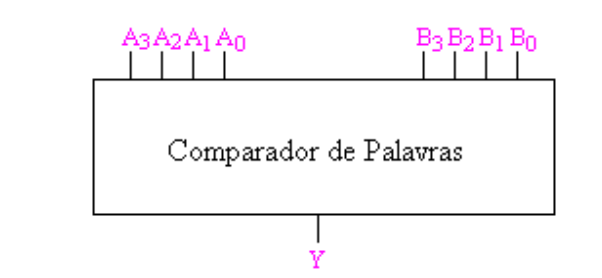
\includegraphics[width=.5\textwidth]{cc1.png}	
\end{figure}

Um comparador tem como saída 1 se os comprimentos forem iguais,caso
contrário a saída sera 0.
Ele também pode possuir três saídas:

\begin{itemize}
	\item	se A=B
	\item	se A\textless B
	\item	se A\textgreater B
\end{itemize}

Para uma boa realização de um circuito combinacional é necessário seguir alguns
passos,como os mostrados abaixo:

\begin{enumerate}[label=(\alph*)]
	\item	Descrever sistema;
	\item 	Elaborar tabela da verdade;
	\item	Obter funções booleanas a partir da tabela verdade;
	\item	Simplificar funções booleanas obtidas ;
	\item	Elaborar diagrama lógico.
\end{enumerate}
Dessa maneira ,fica mais intuitivo a realização da montagem e análise do circuito.

\section{Procedimentos}
\label{sec:Procedimentos}
Parte 1:
\begin{enumerate}[label=(\roman*)]
	\item	Usando apenas portas NAND de DUAS entradas,projetar um
	comparador de palavras de 3 bits, completar a tabela verdade
	para Ai e Bi e obtenher a equação para Zi ;
	\item	Minimizar a função obtida anteriormente;
	\item	Fazer um diagrama lógico parcial. Implementar e verificar se o
	resultado combina com o resultado da tabela verdade;
	\item	Fazer um diagrama lógico total e implementar;
	\item	Comentar os resultados obtidos.
\end{enumerate}
Parte 2:
\begin{enumerate}[label=(\roman*)]
	\item	Elaborar a  tabela verdade parcial e obter as funções booleanas parciais do  circuito Comparador de 1 bit;
	\item	Fazer uma tabela verdade parcial e obter funções parciais;
	\item	Minimizar a função obtida anteriormente;
	\item	Fazer o diagrama lógico parcial. Implementar e verificar se o
	resultado combina com o resultado da tabela verdade;
	\item	Fazer o diagrama lógico total de acordo com a figura
	abaixo e implementar;
	\begin{figure}	
	\end{figure}
	\item	Comente os resultados obtidos.
\end{enumerate}

\subsection{Multiplexador de 4 entradas}
\label{sec:Mux}

Descrever o experimento realizado. Sempre  que colocar uma figura deve-se explicar o que se pretende que o leitor veja, ou uma análise logo após a figura. 


A Figura~\ref{fig:exemplo} apresenta um exemplo de como usar e citar uma figura.

Aqui temos um exemplo de como citar uma URL na bibliografia~\cite{systemverilog}.
Aqui temos um exemplo de como criar um hiperlink. Veja
\href{https://www.youtube.com/watch?v=EcNxjxKRQ6E}{aqui} um exemplo de vídeo.

Sempre identifique no site do vídeo:
\begin{itemize}
    \item o experimento: Experimento 7;
    \item semestre: 2016-2;
    \item a disciplina: CiC 116351 - Circuitos Digitais - Turma B;
    \item a universidade: Universidade de Brasília (UnB);
    \item os nomes dos componentes do grupo.
\end{itemize}

É apresentado acima como fazer uma listagem não numerada.

\subsection{Demultiplexador}
\label{sec:Demux}

Este é outro item do experimento.
Aqui temos um exemplo de como construir e citar uma tabela, conforme mostrado na Tabela~\ref{tab:resultados}.

\begin{table}[H]
    \centering
    \caption{Expected values of the obtained circuits' attributes.}
    \begin{tabular}{|c|c|c|c|c|c|c|c|}
    \cline{2-7}
    \multicolumn{1}{c}{} & \multicolumn{3}{|c|}{Phase 1} & \multicolumn{3}{c|}{Phase 2} & \multicolumn{1}{c}{} \\
    \hline
    Experiment & $n_g$ & $n_l$ & $n_t$ & $n_g$ & $n_l$ & $n_t$ & $t(s)$ \\
    \hline
    1 bit full adder & 8.16 & 3.8 & 47.6 & 5.03 & 3.0 & 25.93 & 99.13 \\
    2 bit full adder & 18.06 & 5.16 & 107.13 & 11.06 & 4.9 & 60.06 & 709.56 \\
    2 bit multiplier & 14.2 & 4.03 & 74.33 & 7.7 & 2.2 & 37.53 & 357.76 \\
    7 segment decoder & 47.53 & 5.83 & 270.46 & 32.86 & 5.0 & 176.4 & 740.63 \\
    Karnaugh 1 bit full adder & 19.0 & 6.0 & 102.0 & 5.03 & 3.0 & 24.8 & 130.73 \\
    \hline
    \end{tabular}
    \label{tab:resultados}
\end{table}

Aqui devemos colocar uma apresentação e análise da tabela, explicando ao leitor o que se pretende mostrar.

\section{Análise dos Resultados}
\label{sec:Resultados}

Faça uma análise crítica dos resultados obtidos nos experimentos. Esta análise pode ser feita item a item ou de uma forma geral.

Dica: Use pesquisa na Internet para tirar as dúvidas sobre edição em \LaTeX .

\section{Conclusão}
\label{sec:Conclusao}
Foi estudado nesse relatório o uso de comparadores de bits, bem como o uso da
ferramenta Quartus II para a implementação de circuitos. Foram usados métodos
conhecidos da síntese de circuitos combinacionais já vistos em aulas teóricas.
Pode-se afirmar que, com a semelhança dos resultados nas tabelas verdades com
as tabelas do Quartus II que foi um experimento de bastante sucesso.
\newpage 
% Colocar aqui apenas as respostas dos itens da Auto-Avaliação
\section*{Auto-Avaliação}

\begin{enumerate}
    \item b
    \item d
    \item d
    \item b
    \item b
\end{enumerate}


\end{document}
